\chapter{DEFINIR}
El presente capítulo desarrolla la segunda etapa del Design Thinking: Definir. Su propósito es sintetizar la información recopilada durante la fase de Empatizar para construir un planteamiento del problema claro y orientado al usuario, formulando un Point of View (POV) que guíe las decisiones de diseño en las etapas subsiguientes (Vargas Márquez et al., 2021). Para ello se aplicaron cuatro técnicas, a partir de las plantillas de Design Thinking en Español: Perfil de Usuario, Mapa de Empatía, Mapa (o Matriz) de Motivaciones y la técnica ¿Cómo podríamos...?

\section{PERFIL DE USUARIO}
Con el objetivo de contar con una referencia clara de los usuarios entrevistados durante las siguientes fases del proyecto, se elaboró un perfil individual para cada participante, sintetizando su biografía, objetivos, personalidad y frustraciones. Esta técnica consiste en elaborar una ficha por cada usuario con el que se interactuó durante la investigación, con una descripción de sus hábitos y necesidades, de modo que el equipo pueda evaluar en cada paso si las ideas desarrolladas se ajustan a los perfiles definidos (Design Thinking en Español, s.f.-g). A continuación, se presentan los perfiles de los Usuarios 1 y 5, seleccionados por representar dos formas distintas de experimentar la desconexión emocional: una vinculada a la dificultad de iniciar vínculos (introversión), y otra vinculada a la cautela derivada de experiencias relacionales previas.

\subsection{Usuario 1}
\begin{figure}[htbp]
  \centering
  \caption{Perfil de usuario - Usuario 1}
  \label{fig:perfil_usuario1}
  \vspace{4pt}
  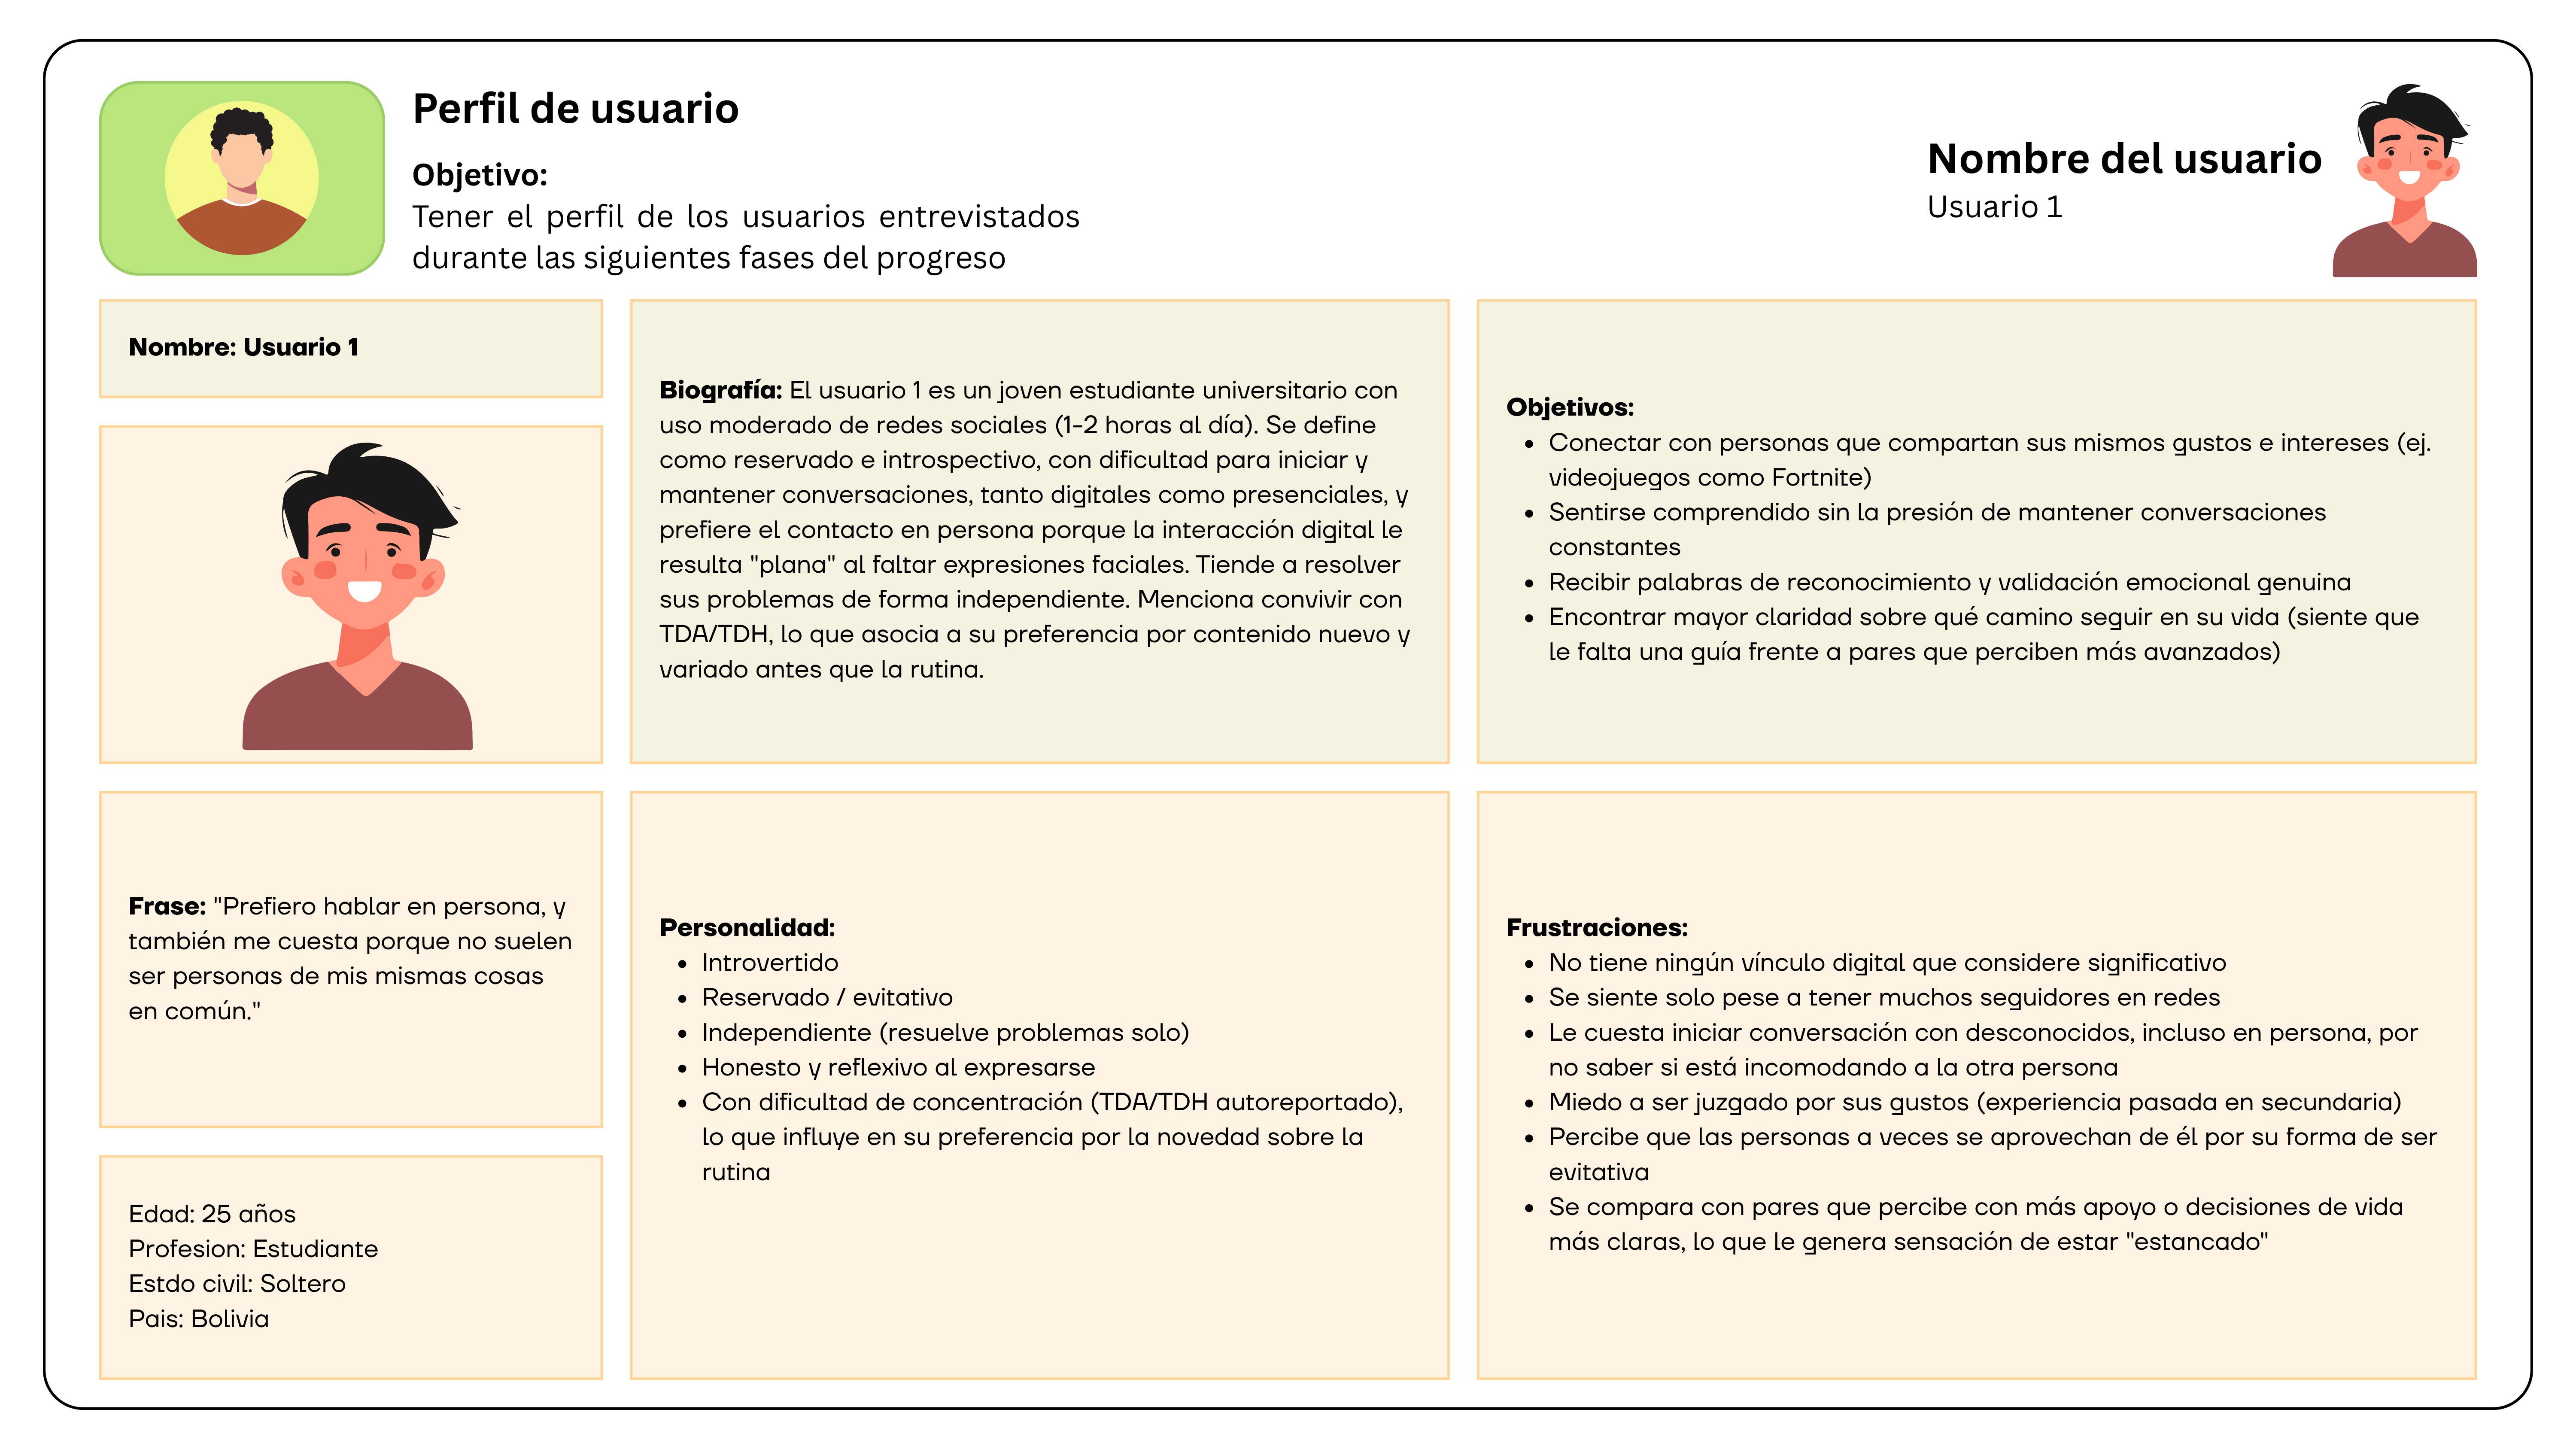
\includegraphics[width=0.9\textwidth]{Images/methodology/define/usuario1P.png}
  \vspace{4pt}
\end{figure}

El perfil del Usuario 1 ilustra un patrón de aislamiento emocional pese a la conectividad digital, consistente con la definición de soledad de Hawkley y Cacioppo (2010), centrada en la percepción de que las necesidades sociales no están siendo satisfechas, especialmente por la calidad de las relaciones. Su frustración central, no tener ningún vínculo digital que considere significativo, refleja de forma individual la experiencia de sentirse rodeado de contactos y, al mismo tiempo, emocionalmente aislado, descrita por Parry et al. (2026).

\subsection{Usuario 5}
\begin{figure}[htbp]
  \centering
  \caption{Perfil de usuario - Usuario 5}
  \label{fig:perfil_usuario5}
  \vspace{4pt}
  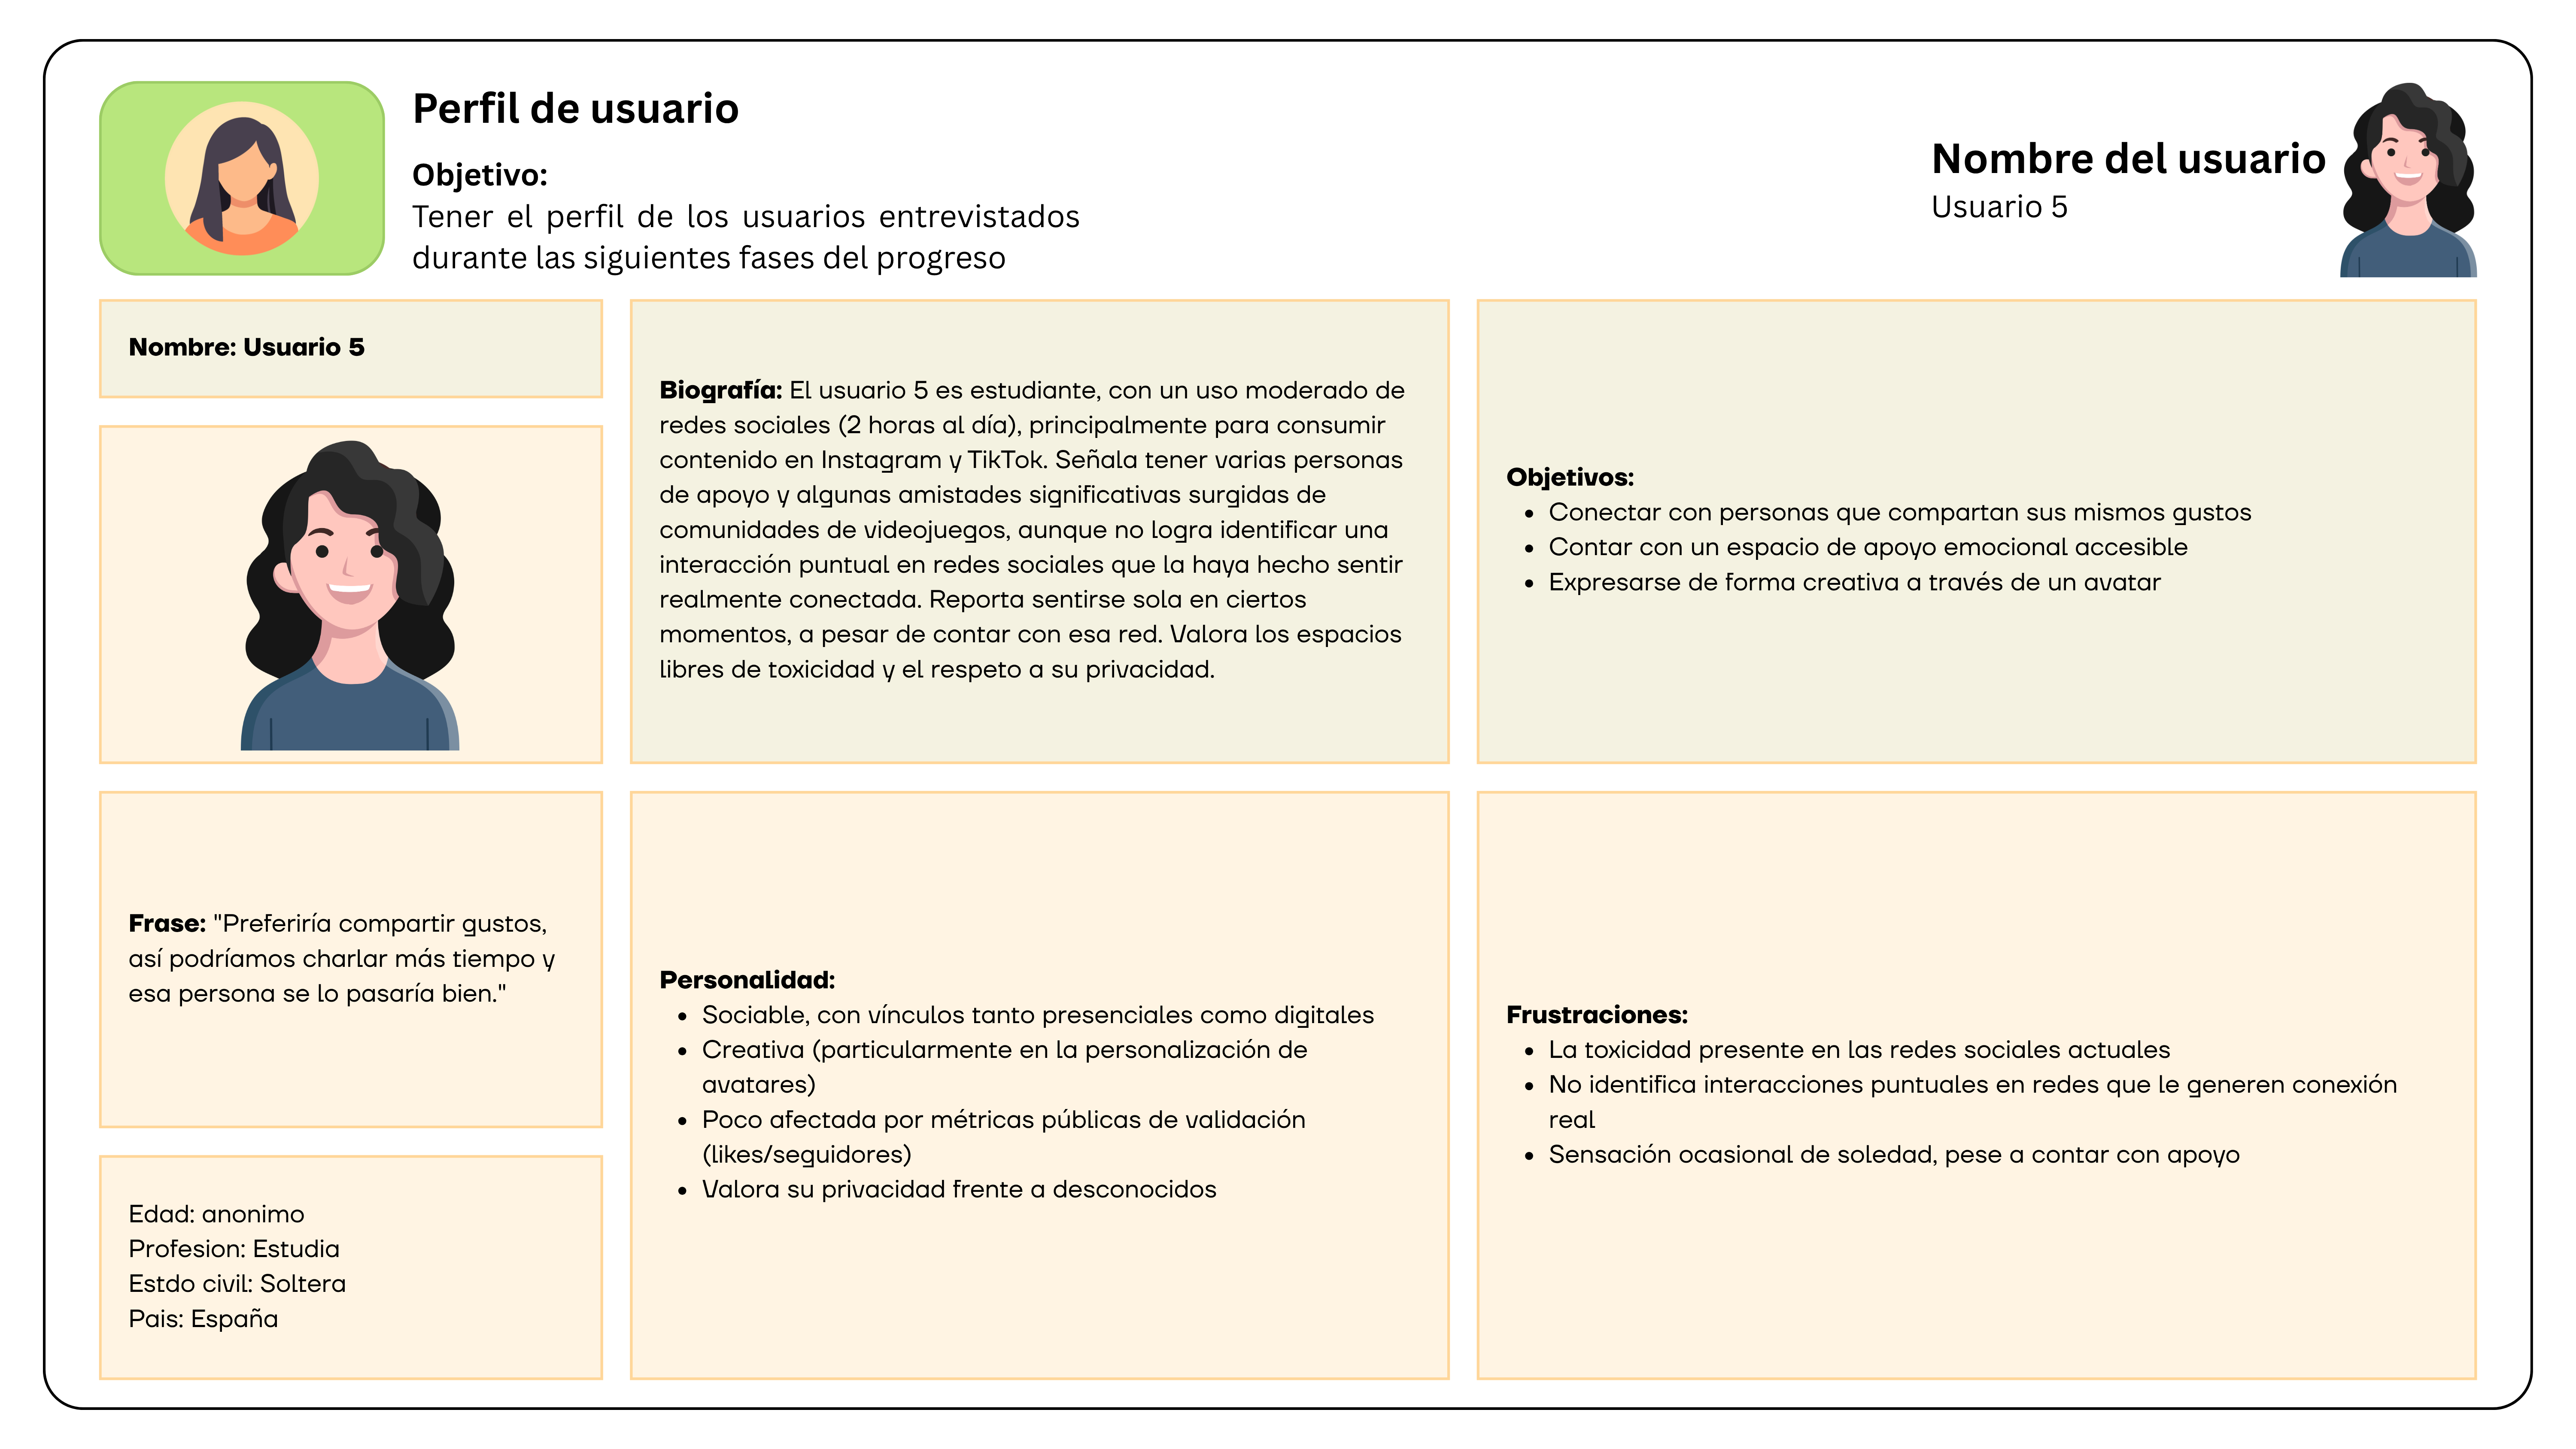
\includegraphics[width=0.9\textwidth]{Images/methodology/define/usuario5P.png}
  \vspace{4pt}
\end{figure}

El perfil del Usuario 5 aporta un matiz relevante al planteamiento del problema: a diferencia del Usuario 1, cuenta con vínculos significativos previos, surgidos de comunidades de videojuegos, lo que respalda el emparejamiento por intereses compartidos como mecanismo de vinculación, en coherencia con la evidencia meta-analítica sobre el papel de la similitud en la atracción interpersonal (Montoya et al., 2008). Sin perjuicio de ello, su experiencia de cautela relacional evidencia que la calidad del vínculo depende también de la gestión emocional de la interacción, y no únicamente de la afinidad temática.

\subsection{Usuarios 2, 3, 4 y 6}
De manera complementaria, se elaboraron los perfiles de los Usuarios 2, 3, 4 y 6. El Usuario 2 se describe como pesimista y reservado al iniciar una interacción (``no inicio conversaciones, depende, a veces pasa o no, soy pesimista porque soy solitario o lo fui''); el Usuario 3 condiciona la conversación a la existencia de un interés común (``con una cosa en común sí se puede hablar y hacerlo entretenido; sin nada en común es difícil conversar''); el Usuario 4, a diferencia del resto, cuenta con una red de apoyo sólida y busca principalmente conectar con personas de gustos muy específicos (``prefiero pocas conversaciones, pero que sean significativas''); y el Usuario 6 enfatiza la dificultad de encontrar personas afines (``me gustaría que fuera con los mismos gustos, siento que sería más fácil entablar una conversación''). En conjunto, estos perfiles refuerzan los hallazgos ya descritos: predominio del consumo pasivo, escasez de vínculos digitales significativos, y una valoración compartida hacia mecanismos de emparejamiento por afinidad y personalización mediante avatares.

\section{MAPA DE EMPATÍA}
Con el objetivo de sistematizar visualmente lo que cada usuario piensa, siente, escucha, ve, habla y hace, así como sus dolores y necesidades, se elaboró un Mapa de Empatía por participante, a partir de la información recogida en las entrevistas. Esta técnica permite comprender y plasmar las necesidades, deseos, motivaciones y experiencias de los usuarios; aunque suele asociarse a la fase de Empatía, se recomienda realizarla en la fase de Definición, cuando ya se cuenta con la información de la investigación de usuarios, para no basarla en suposiciones (Design Thinking en Español, s.f.-e).

\subsection{Usuario 1}
\begin{figure}[htbp]
  \centering
  \caption{Mapa de empatía - Usuario 1}
  \label{fig:mapa_empatia_usuario1}
  \vspace{4pt}
  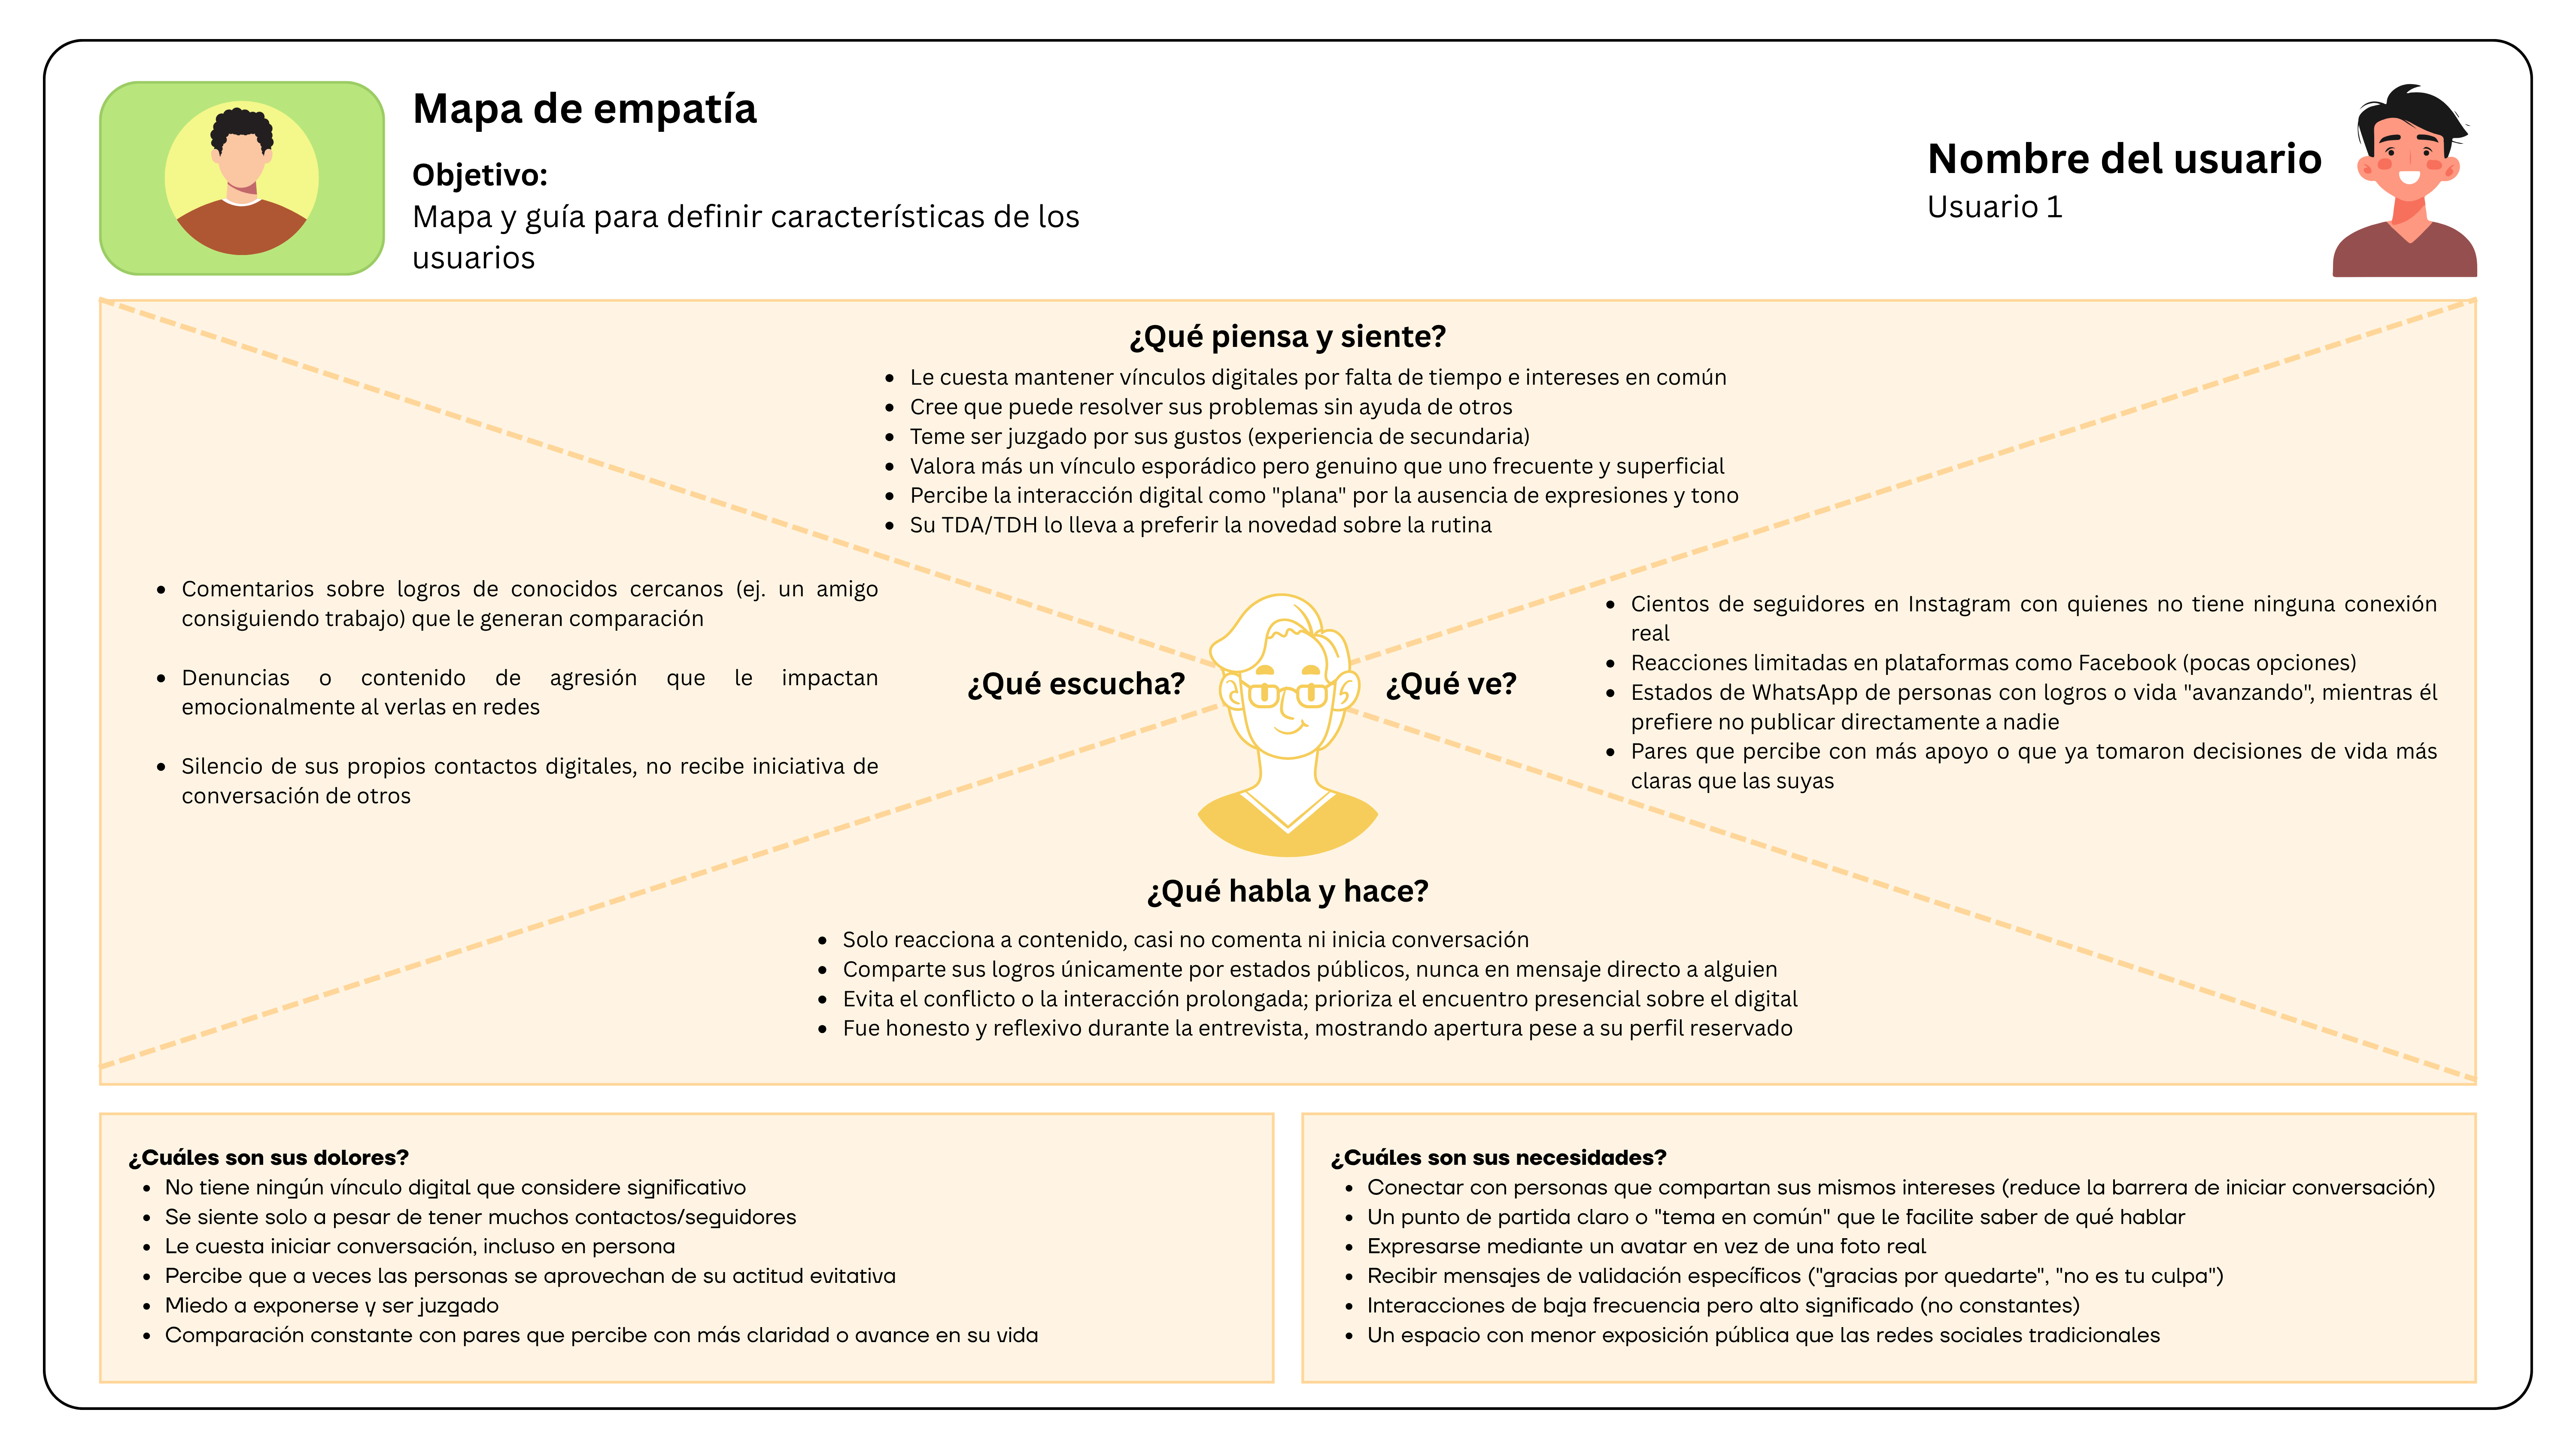
\includegraphics[width=0.9\textwidth]{Images/methodology/define/usuario1ME.png}
  \vspace{4pt}
\end{figure}

El mapa evidencia que la percepción de la comunicación digital como "plana", debido a la ausencia de expresiones y tono de voz, constituye un dolor central para el Usuario 1, lo que resulta coherente con la observación de Picard (1997) de que la comunicación textual prescinde de la entonación de la voz y de la expresión facial (p. 13).

\subsection{Usuario 5}
\begin{figure}[htbp]
  \centering
  \caption{Mapa de empatía - Usuario 5}
  \label{fig:mapa_empatia_usuario5}
  \vspace{4pt}
  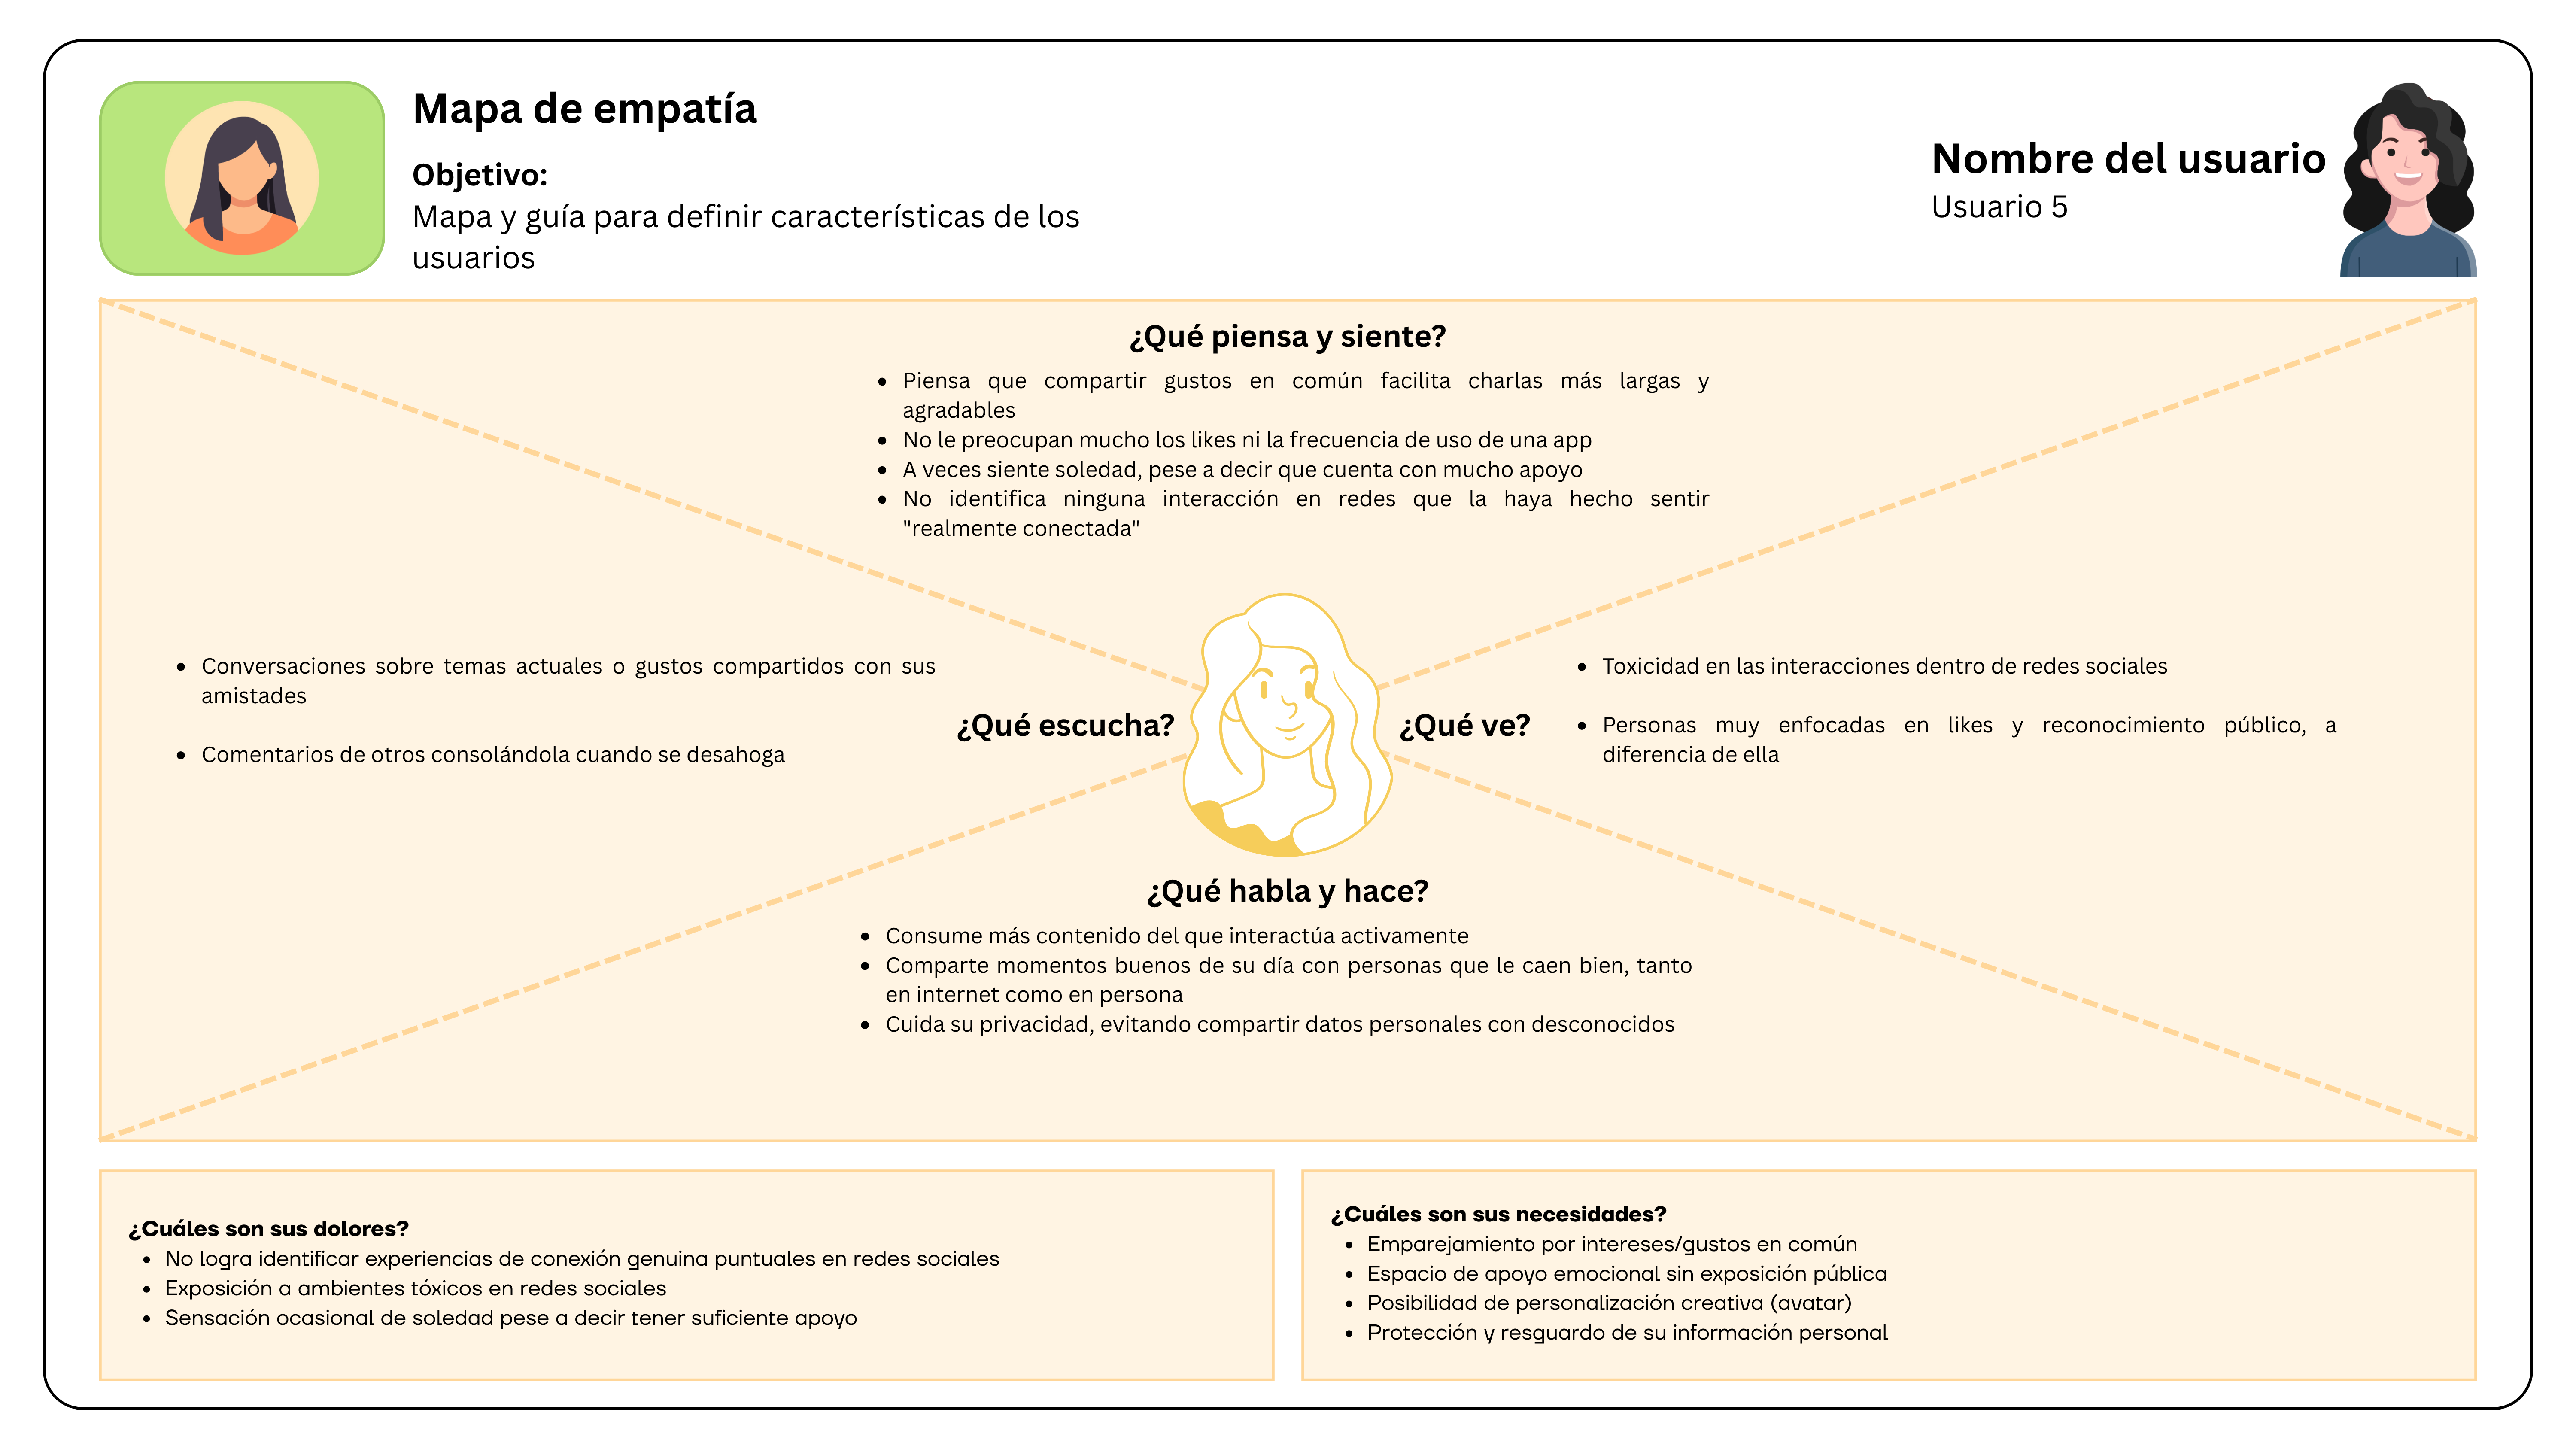
\includegraphics[width=0.9\textwidth]{Images/methodology/define/usuario5ME.png}
  \vspace{4pt}
\end{figure}

En el caso del Usuario 5, el mapa revela una necesidad de protección de la privacidad frente a desconocidos como condición previa para la confianza, lo que resulta coherente con los mecanismos de seguridad y moderación contemplados en el alcance del proyecto.

\subsection{Usuarios 2, 3, 4 y 6}
Los Mapas de Empatía correspondientes a los Usuarios 2, 3, 4 y 6 confirman de forma reiterada los mismos dolores y necesidades: escasos vínculos digitales significativos, exposición a ambientes hostiles o de comparación social, y una necesidad compartida de espacios que prioricen la calidad de la interacción sobre la exposición pública. Entre los matices de cada mapa destacan el trato hostil hacia personas nuevas en comunidades en línea y la presión de las métricas cuando actúa como creador de contenido (Usuario 2); los ambientes conflictivos y el temor a la traición al confiar en alguien nuevo (Usuario 3); la exposición a estándares de belleza irreales y la necesidad de un formato de mensaje que no limite su expresión (Usuario 4); y el temor por la seguridad al interactuar con desconocidos, junto con la comparación frente al éxito ajeno (Usuario 6).

\section{MAPA DE MOTIVACIONES}
Con el objetivo de identificar variables positivas compartidas entre los distintos usuarios respecto a sus necesidades, se elaboró un Mapa de Motivaciones cruzando la información de los seis participantes entrevistados. Esta técnica se materializa en una matriz en la que aparecen todos los usuarios y, en cada intersección, se definen las motivaciones que los conectan; se aplica en la fase de Definición, a partir de la información obtenida en la fase de Empatía (Design Thinking en Español, s.f.-f).

\begin{figure}[htbp]
  \centering
  \caption{Mapa de motivaciones}
  \label{fig:mapa_motivaciones}
  \vspace{4pt}
  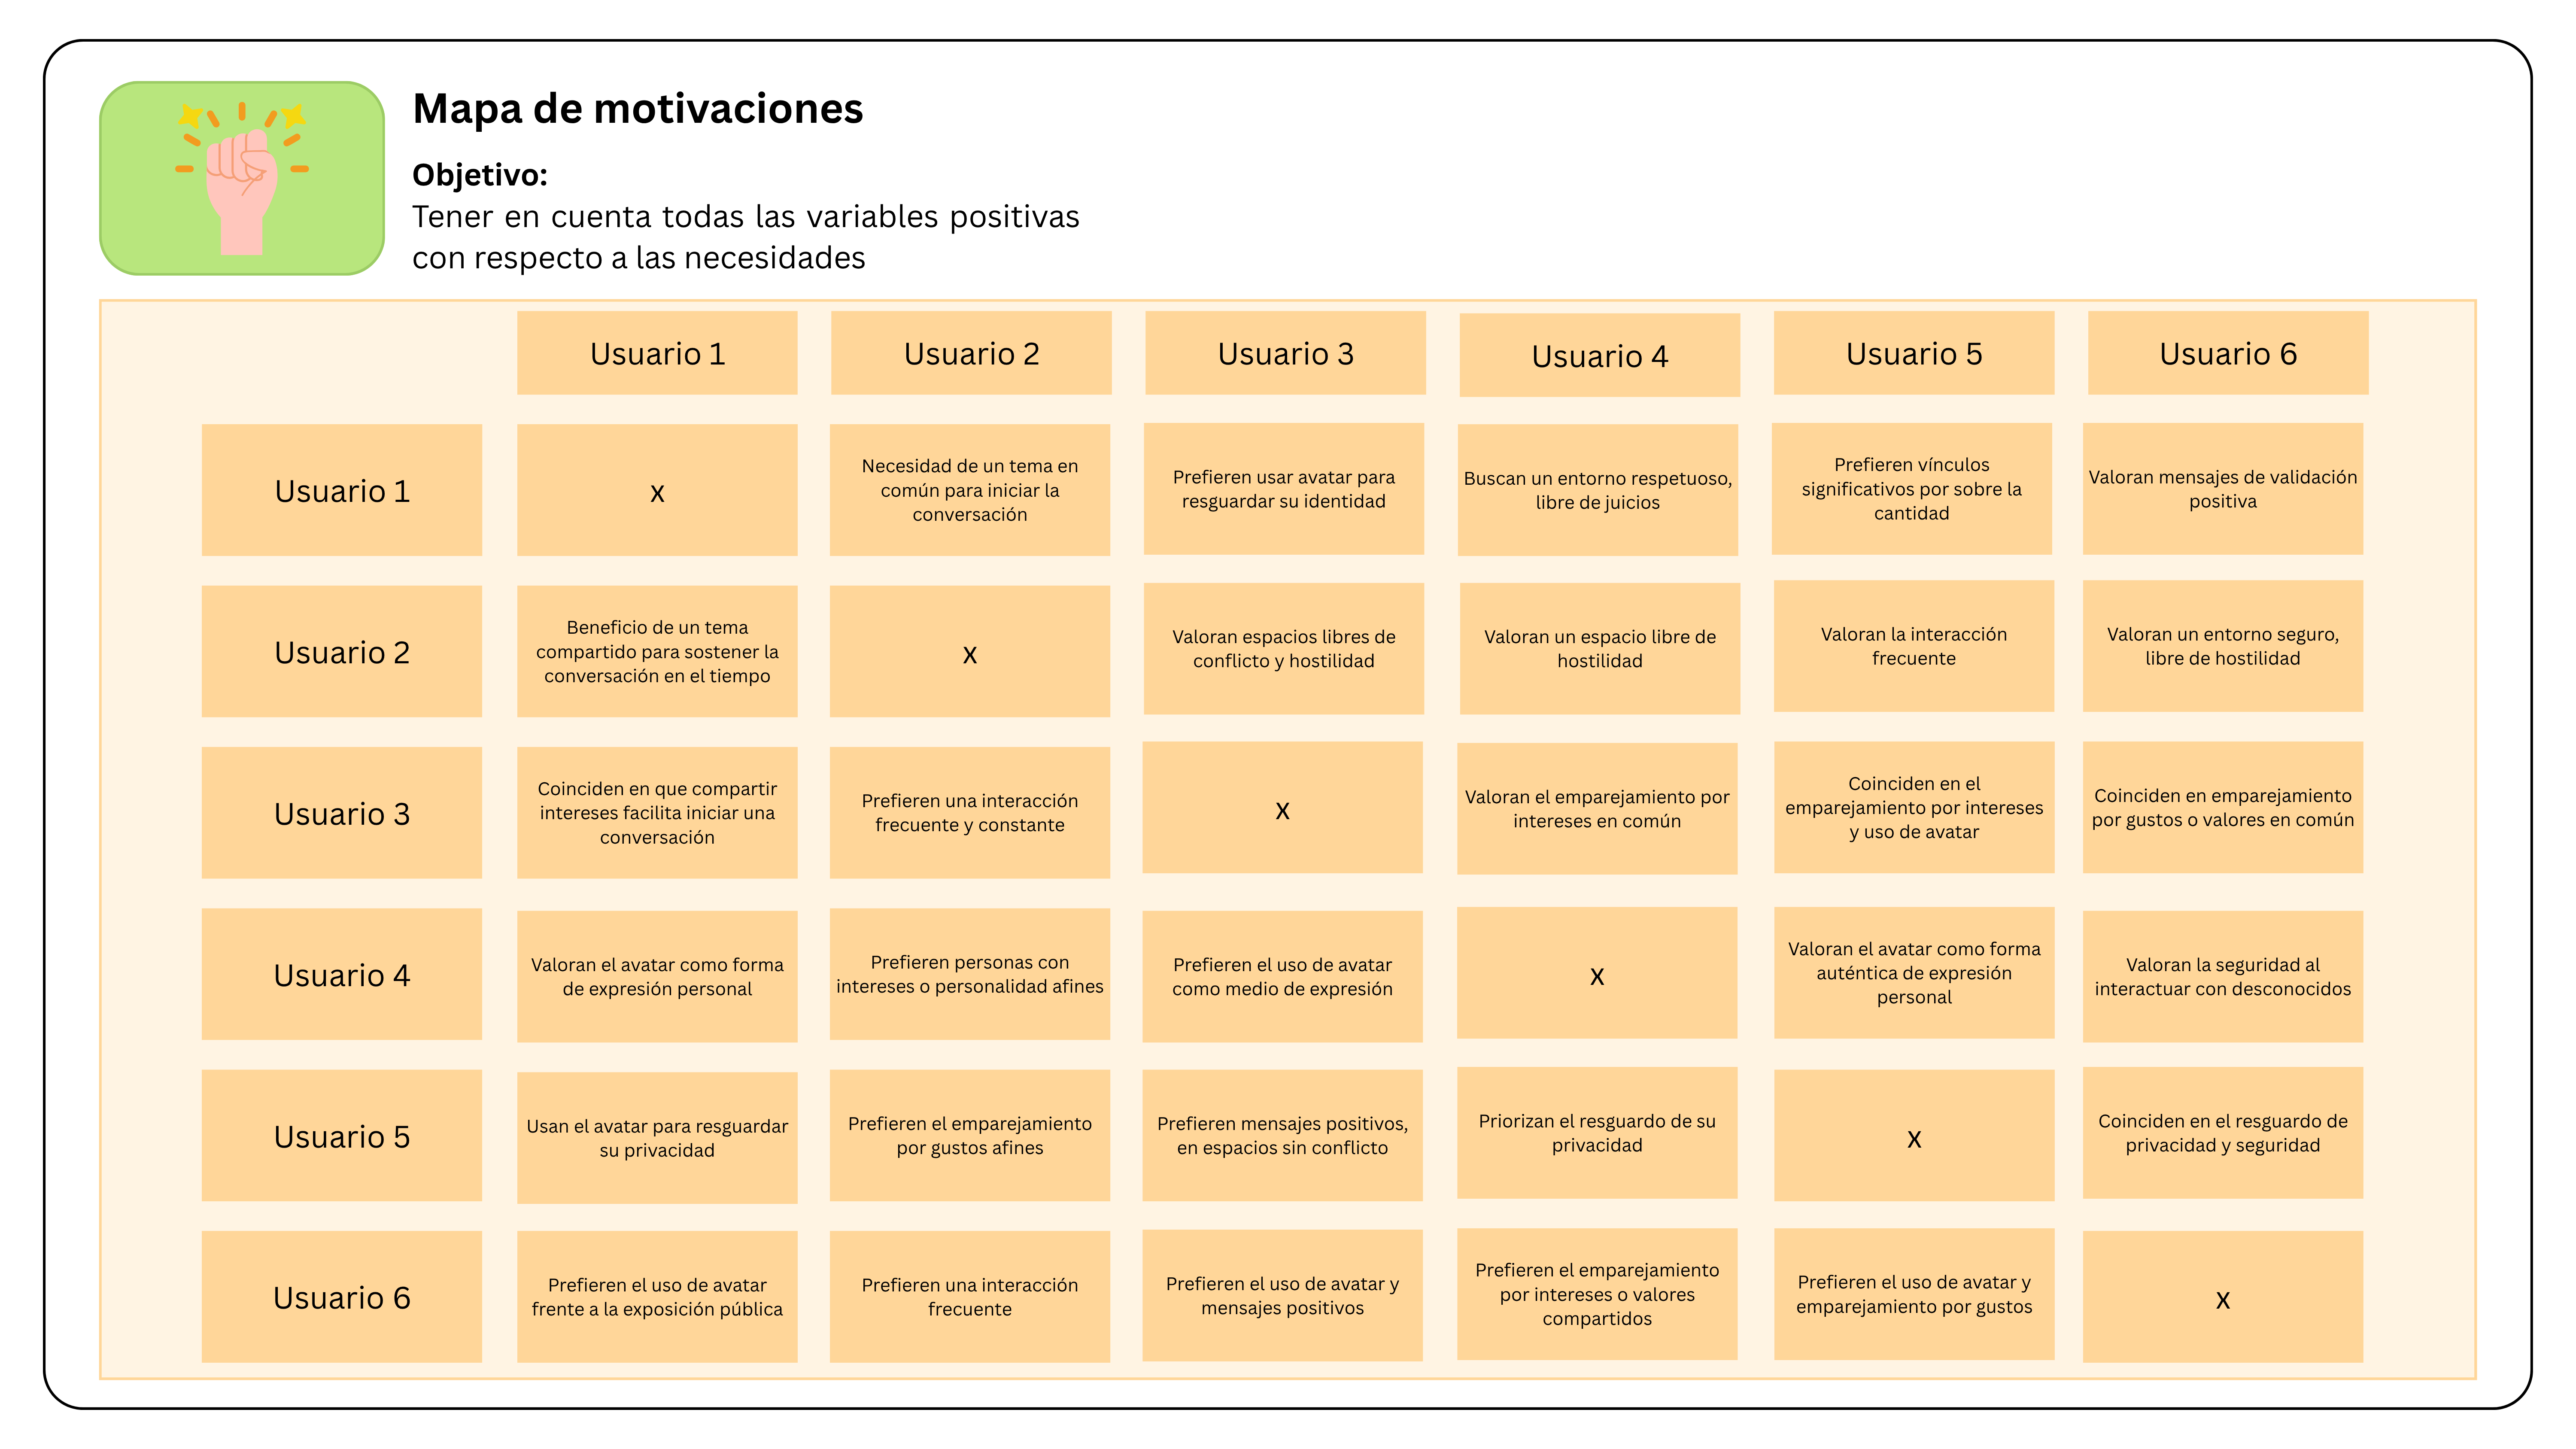
\includegraphics[width=0.95\textwidth]{Images/methodology/define/mapaDeMotivaciones.png}
  \vspace{4pt}
\end{figure}

Con seis participantes, la matriz contiene 15 pares posibles, cada uno representado por dos celdas. El análisis cruzado de estos pares permitió identificar tres motivaciones predominantes: (a) la necesidad de un interés o gusto en común como facilitador de la conversación, presente en 9 de los 15 pares; (b) la preferencia por el uso de un avatar como medio de expresión o de resguardo de la identidad, presente también en 9 de los 15 pares; y (c) la necesidad de un entorno seguro, respetuoso o libre de hostilidad, presente en 8 de los 15 pares (5 referidos a la ausencia de conflicto u hostilidad y 3 a la seguridad y la privacidad frente a desconocidos). Con menor frecuencia aparecieron la preferencia por una interacción frecuente (3 pares), por mensajes positivos o de validación (3 pares) y por vínculos significativos antes que numerosos (1 par). Estos hallazgos, obtenidos de forma inductiva a partir de la evidencia primaria, coinciden con los factores identificados deductivamente a partir de la literatura en el Capítulo 4, en particular con los planteamientos de Godard y Holtzman (2024) sobre el valor del uso activo, con la evidencia sobre la similitud como base de la atracción interpersonal (Montoya et al., 2008), y con los hallazgos de Burke y Kraut (2016) sobre el papel del tipo de comunicación y de la fuerza del vínculo en el bienestar.

\section{¿CÓMO PODRÍAMOS...?}
A partir de los conocimientos sintetizados en el Mapa de Motivaciones, se aplicó la técnica ¿Cómo podríamos...? con el objetivo de convertir dichos hallazgos (insights) en preguntas orientadoras que faciliten la posterior generación de ideas en la etapa de Idear. Estas preguntas constituyen el eslabón entre las áreas de oportunidad identificadas y la generación de ideas, ya que las posibles respuestas a ellas son las ideas que construirán la solución (Design Thinking en Español, s.f.-i).

\begin{figure}[htbp]
  \centering
  \caption{Técnica ¿Cómo podríamos...?}
  \label{fig:como_podriamos}
  \vspace{4pt}
  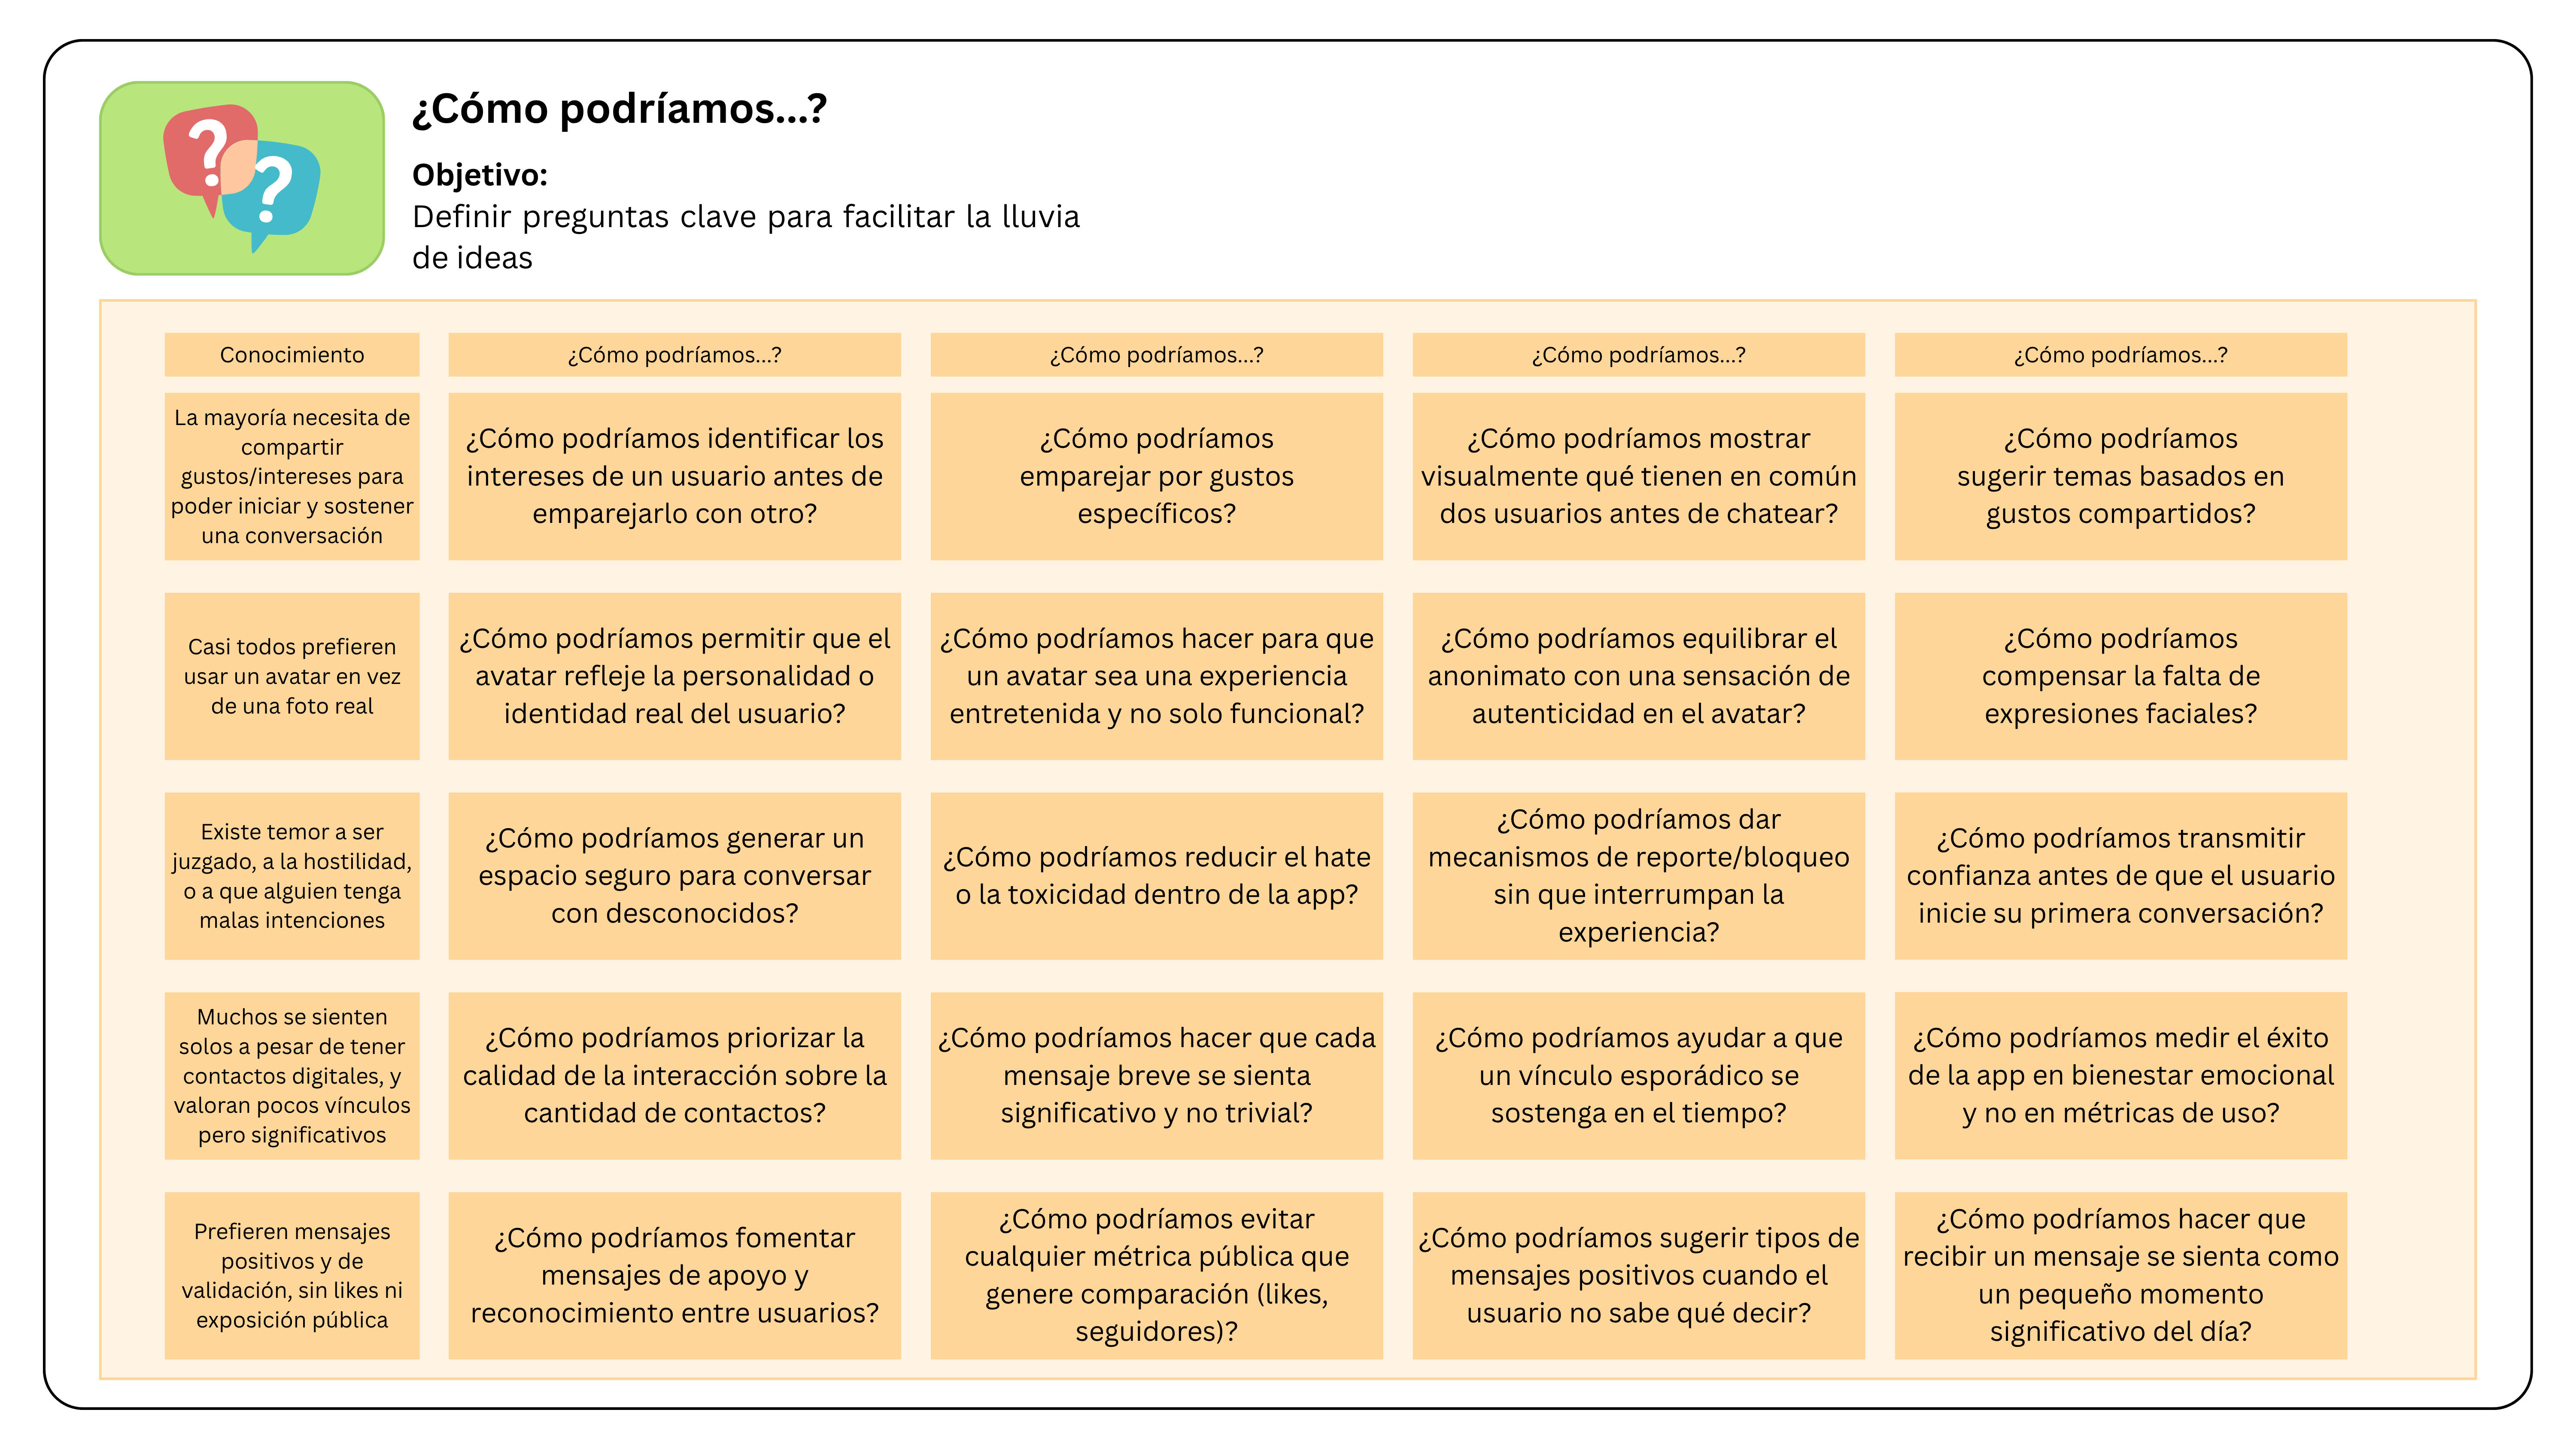
\includegraphics[width=0.95\textwidth]{Images/methodology/define/comoPodriamos.png}
  \vspace{4pt}
\end{figure}

Se formularon cuatro preguntas por cada uno de los cinco conocimientos centrales derivados de la fase de Empatizar, veinte en total, que abordan: la necesidad de intereses compartidos, la preferencia por el uso de avatares, el temor a la hostilidad o a interactuar con desconocidos, la preferencia por vínculos pocos pero significativos, y la preferencia por mensajes positivos libres de métricas públicas de validación. Estas preguntas constituyen el punto de partida directo para la generación de ideas desarrollada en el Capítulo 7.

\section{PLANTEAMIENTO DEL PROBLEMA (POINT OF VIEW)}
A partir de la síntesis de la evidencia documental (Capítulo 4) y de la evidencia primaria recolectada en el presente capítulo, se formula el siguiente planteamiento del problema (POV), en los términos propuestos por Vargas Márquez et al. (2021):

\begin{quote}
Los jóvenes de 16 a 28 años necesitan un espacio digital que priorice la calidad de la interacción sobre la cantidad de conexiones, porque las plataformas actuales, centradas en el consumo pasivo de contenido y en métricas públicas de validación, no logran satisfacer su necesidad de vínculos genuinos, generando una desconexión emocional pese a la hiperconectividad.
\end{quote}

Este planteamiento integra los hallazgos más consistentes de la fase de Empatizar —la necesidad de afinidad temática, la preferencia por el anonimato progresivo mediante avatares, la exigencia de seguridad frente a desconocidos y la preferencia por vínculos escasos pero significativos— y constituye la base sobre la cual se desarrollan las técnicas de generación de ideas en el Capítulo 7.